% Experiment 6: backend/evals/paper/exp6_dispatch.py   (30 seeds)
% Experiment 7: backend/evals/paper/exp7_escrow.py     (30 seeds; frontier 10)
Table~\ref{tab:dispatch} dispatches the same 30 simulated semesters (routine regime,
about 26,000 errands each) in four ways. Each runner's willingness and response delay
for a given errand are fixed by a seed shared across policies, so the policies differ
only in when each runner is told.

\emph{Ranking alone does little.} Ranking a simultaneous broadcast by trust left
17.8\% of errands with a runner within two hops. When every candidate is told at
once, the order of the list cannot change who answers first. Staging the same offers
in time doubled that to 35.8\%, at a cost of 6.7~s in median wait and 42~s at the
90th percentile. Offering to one runner at a time in trust order reached 50.4\% but
more than doubled the median wait again.

\emph{The router creates in-group circulation.} The same table measures the effect
that motivates Section~\ref{sec:design-policy}. Staging doubled the share of an
honest group's errands that stayed inside the group, from 3.5\% to 7.0\%, and
one-at-a-time dispatch raised it to 12.1\%. No group member chose this; the router
did. This is the circulation the ring detector reads, and it is why the detector
must be conditioned on the router.

\emph{The control group is not free.} The 5\% coin is tossed for each logged first
offer, and an errand whose friends-first round finds nobody is tossed again for the
unrestricted round, so 7.0\% of errands went out exploratory. Of those, 12.8\% went
to a runner within two hops, against 37.5\% in regular rounds.

\emph{The scheduler fix.} When a requester has no friend or friend-of-friend among the
five nearest runners, the first offer goes straight to those five. Under the original
scheduler such an errand was never widened, and 4.4\% of them went unaccepted for 30
minutes, which made staged dispatch the only policy with an overall expiry rate of
1.9\%. With the 90-second widening applied to these errands too, their expiry fell
to 0.23\%, the same as the other policies, while the share taken within two hops
moved only from 36.2\% to 35.8\%.

\begin{table}[!t]
\caption{Dispatch Policies on the Same Simulated Semesters.
Mean (95\% CI Half-Width) Over 30 Seeds}
\label{tab:dispatch}
\centering
\scriptsize
\setlength{\tabcolsep}{1.6pt}
\begin{tabular}{@{}lcccc@{}}
\toprule
& Broadcast, & \multicolumn{2}{c}{Staged} & One at \\
\cmidrule(lr){3-4}
& ranked & fixed & original & a time \\
\midrule
Taken within 2 hops (\%) & 17.8 (0.1) & 35.8 (0.2) & 36.2 (0.2) & 50.4 (0.3) \\
By a direct friend (\%) & 5.1 (0.1) & 10.3 (0.1) & 10.4 (0.1) & 18.0 (0.1) \\
Honest group's errands kept inside (\%) & 3.5 (0.1) & 7.0 (0.2) & 7.0 (0.2) & 12.1 (0.3) \\
Median wait (s) & 12.3 (0.0) & 19.0 (0.1) & 18.6 (0.1) & 41.9 (0.1) \\
90th-percentile wait (s) & 36.7 (0.2) & 78.9 (0.1) & 76.8 (0.1) & 122.2 (0.4) \\
Unaccepted after 30 min (\%) & 0.22 (0.01) & 0.22 (0.01) & 1.88 (0.03) & 0.22 (0.01) \\
\quad unrestricted first offer (\%) & n/a & 0.23 (0.02) & 4.38 (0.06) & n/a \\
\bottomrule
\multicolumn{5}{@{}p{0.97\columnwidth}@{}}{``Original'' is the scheduler before the
fix in Section~\ref{sec:impl}. About 40\% of staged errands had no friend or
friend-of-friend among the five nearest runners and went out unrestricted.}
\end{tabular}
\end{table}

\emph{Escrow.} We drew 3,000 orders per seed, mixing MRP goods with one to four
loose-priced lines, and assumed that a loose item costs its listed price 70\% of the
time and 10\%, 20\% or 35\% more otherwise. Each line was judged by the production
judge and each hold computed by the production ledger code. With no headroom,
56\% of payouts would freeze for review. Fig.~\ref{fig:escrow} traces the trade-off
as the headroom grows. For about the same money locked without need (Rs.~17--18 per
order), headroom on loose-priced items alone froze 3.5\% of payouts against 7.0\% for
headroom on the whole order, and full protection needed Rs.~39 against Rs.~87. The
deployed 16\% froze 9.0\% (95\% CI $\pm0.2$) of payouts while locking Rs.~12.7 per
order. Under a dearer price model, in which half of all loose items cost 10--60\%
more than listed, it froze 18.4\%, and the advantage of targeting the uncertain part
held along the whole curve. The same headroom bounds the cold-start case of
Section~\ref{sec:design-reference}: an unpriced line can be over-claimed only up to
the slack in the hold, Rs.~12.7 per order on average and Rs.~32 at the 95th
percentile here, before the payout freezes for a person to look at.

\begin{figure}[!t]
\centering
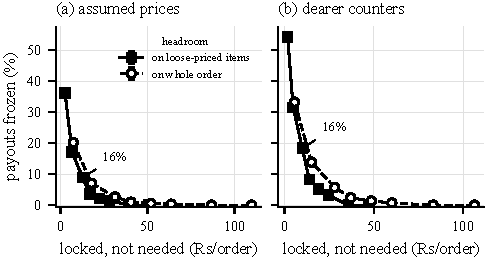
\includegraphics[width=\columnwidth]{figures/fig_escrow.pdf}
\caption{Payouts frozen for review against money locked without need, as escrow
headroom rises from 5\% to 50\%, for two choices of what the headroom covers, under
(a) the assumed price model and (b) a dearer one. Error bars are 95\% confidence
intervals over 10 seeds of 3,000 orders.}
\label{fig:escrow}
\end{figure}
